\section{Theoretical Analysis}
\label{sec:analysis}

In this section, the circuit shown in Figure \ref{fig:t5} is analysed 
theoretically.

The Transfer Function is given by the following equation,

\begin{equation} \label{eq1}
T=\frac{R_1 C_1 s}{1+R_1 C_1 s}(1+ \frac{R_2}{R_1} \frac{1}{1+R_2 C_2 s})
\end{equation}
where $s=2\pi f \times j$.

The frequency of the low pass filter part of the circuit is computed as

\begin{equation} \label{eq2}
\omega_L=\frac{1}{R_2 C_2}
\end{equation}

and the frequency of the high pass filter part of the circuit is given by

\begin{equation} \label{eq3}
\omega_H=\frac{1}{R_1 C_1}
\end{equation}

This leads to a central frequency expressed as

\begin{equation} \label{eq4}
\omega_C=\sqrt{\omega_L \times \omega_H}
\end{equation}

Dividing the value obtained from equation \ref{eq4} by $2\pi$, we get one of the values of interest of the circuit, which should be of $1 kHz$. \par

\begin{table}[h]
  \centering
  \begin{tabular}{|l|r|}
    \hline    
    {\bf Name} & {\bf Value [Hz]} \\ \hline
    $Z_{I1}$ & 640.4922\\ \hline
$Z_{O1}$ & 477.0475\\ \hline
$AV_{1}$ & 110.6998\\ \hline
$Z_{I2}$ & 15013.86\\ \hline
$Z_{O2}$ & 0.9327305\\ \hline
$AV_{2}$ & 0.9856738\\ \hline

  \end{tabular}
  \caption{Frequencies}
  \label{tab:data}
\end{table}
\FloatBarrier


The gain of the circuit is given by the formula below,

\begin{equation} \label{eq5}
Gain = |\frac{R_1 C_1 \omega_C j}{1+R_1 C_1 \omega_C j} \times (1+\frac{R_3}{R_4}) \times \frac{1}{1+R_2 C_2 \omega_C j}|
\end{equation}

Also, the input impedance is given by

\begin{equation} \label{eq6}
Z_{in}=|R_1 + \frac{1}{j \omega_C C_1}|
\end{equation}

and the output impedance as

\begin{equation} \label{eq7}
Z_{out}=|\frac{1}{j \omega_C C_2+\frac{1}{R_2}}|
\end{equation}

\begin{table}[h]
  \centering
  \begin{tabular}{|l|r|}
    \hline    
    {\bf Name} & {\bf Value [dB]} \\ \hline
    $Z_{I}$ & 640.4922\\ \hline
$Z_{O}$ & 2.9364\\ \hline
$AV$ & 107.21838\\ \hline

  \end{tabular}
  \caption{Gain and impedances}
  \label{tab:data2}
\end{table}
\FloatBarrier

%Dizer que são apresentados os gráficos do output voltage gain e tambem da phase. Acho que é tudo
\begin{figure}[h] \centering
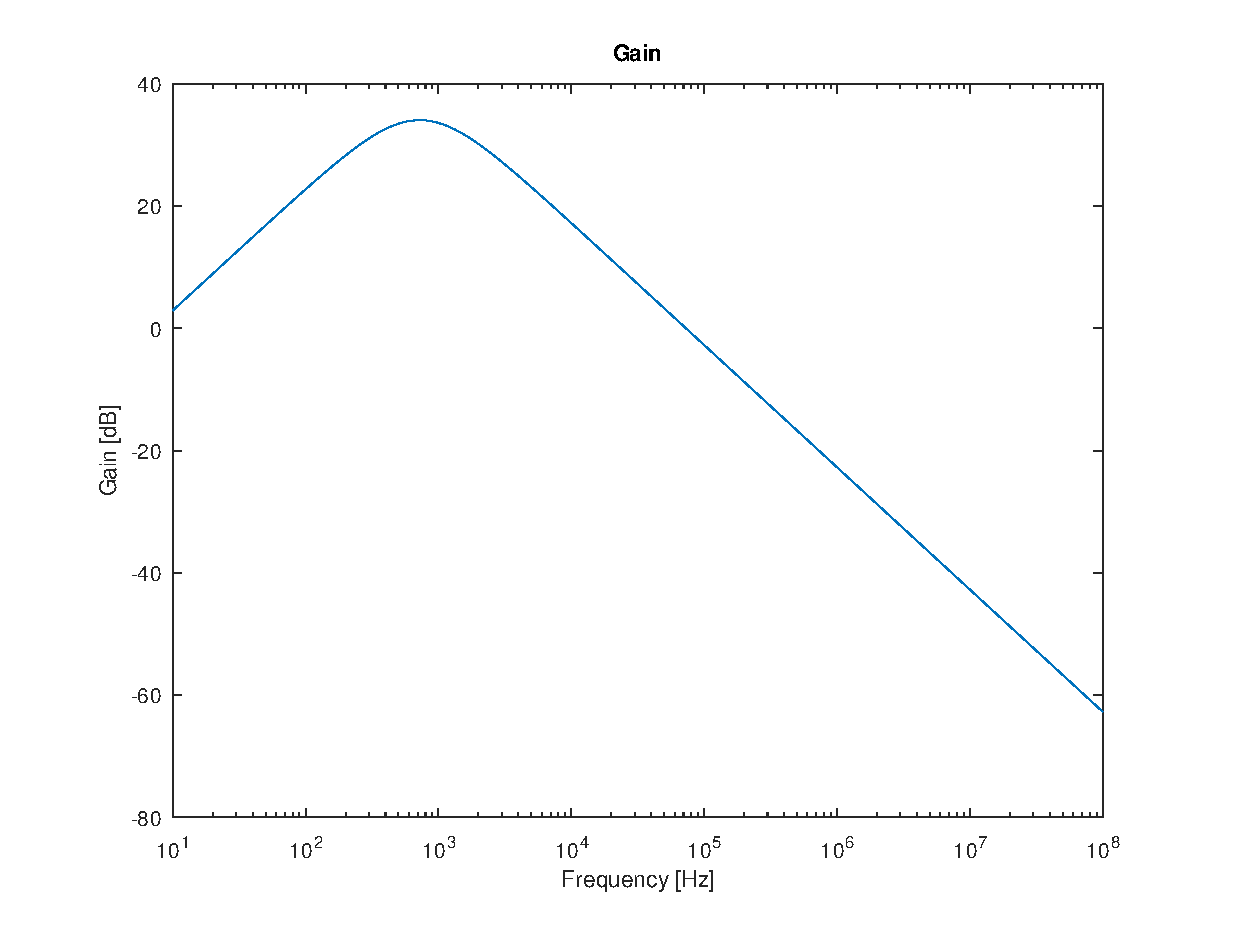
\includegraphics[width=0.6\linewidth]{teo_gain.eps}
\caption{Output voltage gain in order to frequency}
\label{fig:gain}
\end{figure}
\FloatBarrier

\begin{figure}[h] \centering
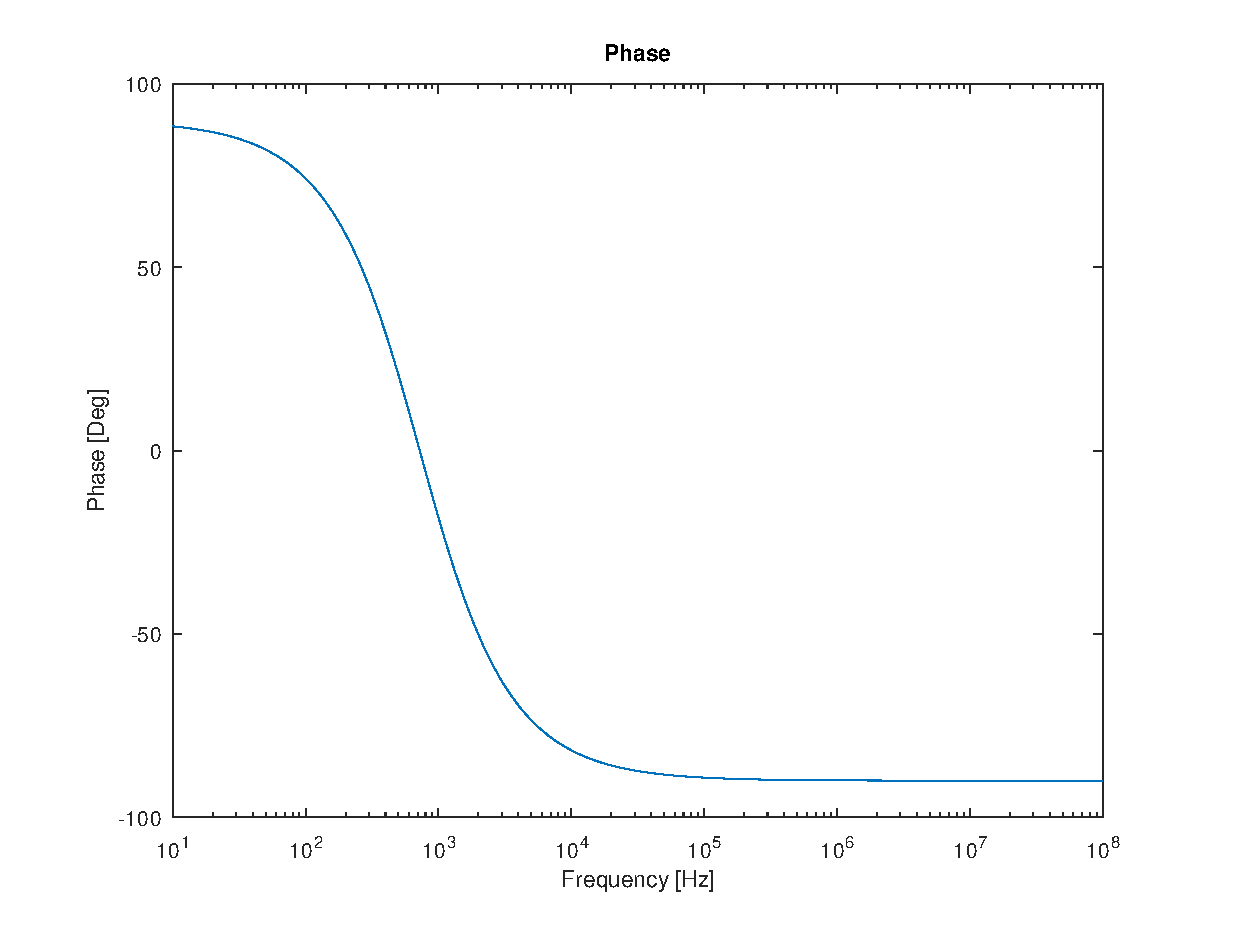
\includegraphics[width=0.6\linewidth]{teo_phase.eps}
\caption{Phase in order to frequency}
\label{fig:phase}
\end{figure}
\FloatBarrier

Here we present the merit figure of our circuit.

\begin{table}[h]
  \centering
  \begin{tabular}{|l|r|}
    \hline    
    {\bf Name} & {\bf Value [Hz] [Mu]} \\ \hline
    \input{../mat/data3_teo}
  \end{tabular}
  \caption{Merit figure}
  \label{tab:data3}
\end{table}
\FloatBarrier



